\documentclass[twocolumn]{article}

%%% PACKAGES %%%
\usepackage[a4paper, margin=0.75in]{geometry}
\usepackage{setspace}
\usepackage{authblk}
\usepackage{graphicx}
\usepackage{float}
\usepackage{stfloats}
\usepackage{blindtext}
\usepackage{caption}
\usepackage{titlesec}
\usepackage{svg}
\usepackage{enumitem}
\usepackage{tikz}
\usetikzlibrary{arrows, arrows.meta, calc, positioning, quotes, shapes}
\usepackage{amsmath}
\usepackage{amssymb}

%%% CONFIG %%%
\renewcommand{\thesection}{\Alph{section}}
\renewcommand{\thesubsection}{\arabic{subsection}}
\titleformat{\section}{\centering\large\bfseries}{Part \thesection}{0em}{}{}
\titleformat{\subsection}{\bfseries}{\thesubsection.}{0.5em}{}{}
\setlist[enumerate]{
    label=(\alph*),
    wide=0pt,
}
\setlength{\abovecaptionskip}{5pt}
\setlength{\belowcaptionskip}{0pt}

%%% TITLE METADATA %%%
\title{CSC311 Final Report: Project Option 1}
\author[]{Leo Peckham}
\author[]{Longyue Wang}
\author[]{Gursewak Sandhu}
\affil[]{}
\date{}

\begin{document}
\maketitle

\section{}

\subsection{$k$-nearest neighbours}

\begin{enumerate}

\item
~
\begin{figure}[!h]
    \centering
    \includesvg[width=\linewidth]{A1a}
    {\footnotesize
        \setlength{\tabcolsep}{3pt}
        \begin{tabular}{ |c|c|c|c|c|c|c| } 
            \hline
            \textbf{$k$-value} & 1 & 6 & {\bf 11} & 16 & 21 & 26 \\ 
            \textbf{Accuracy} & 0.628 & 0.677 & {\bf 0.689}
                              & 0.675 & 0.668 & 0.651 \\ 
            \hline
        \end{tabular}
    }
    \captionof{figure}{Accuracies of user-clustering {\sc knn}}
    \label{fig:userclustering}
\end{figure}


\item
From this data, we can see that the $k^*$ that gave us the best validation
accuracy was $k^* = 11$. Running on test we achieve an accuracy of $0.683$.

\item
~
\begin{figure}[H]
    \centering
    \includesvg[width=\linewidth]{A1c}
    {\footnotesize
        \setlength{\tabcolsep}{3pt}
        \begin{tabular}{ |c|c|c|c|c|c|c| } 
            \hline
            \textbf{$k$-value} & 1 & 6 & 11 & 16 & {\bf 21} & 26 \\ 
            \textbf{Accuracy} & 0.618 & 0.660 & 0.680
                              & 0.687 & {\bf 0.690} & 0.689 \\ 
            \hline
        \end{tabular}
    }
    \captionof{figure}{Accuracies of question-clustering {\sc knn}}
    \label{fig:questionclustering}
\end{figure}

Question-based clustering assumes that if two questions have very similar
distributions of answers across the known students, then the questions will
behave similarly for new students. Intuitively, if two questions ask about a
specific theorem, then the same students who get the first one wrong because
they forgot the statement of the theorem will get the second wrong as well.

From the data in Figure \ref{fig:questionclustering}, we can see that the $k^*$ that gave us the best validation
accuracy was $k^* = 21$. Running on test we achieve an accuracy of $0.670$.

\item
The performances across the board are similar. The user-based approach does
better on test, but only by around a tenth of a percent accuracy. The graphs
for different $k$-values do look quite different, though, with the
user-clustering in Figure \ref{fig:userclustering} falling off much faster for
high $k$-values than the question-clustering in figure
\ref{fig:questionclustering} .

\item

This method relies on a sufficient amount of data to be able to accurately
cluster. If there is an example with a significant amount held-out, it will
become inaccurate because many nearby users/questions will look similar.

The dimension of the features is also a problem. First, it can be extremely
high, being either the number of students or the number of questions. This
poses a problem for a {\sc knn} approach, especially one that uses a Euclidean
distance like this one. Mapping to a smaller latent space first and using
another distance function would help alieviate this problem. Second, if we add
new students or questions to the dataset, the very {\it dimensionality} of our
data will change. This makes it more difficult to improve our model with new
data; mapping to a laten space would also fix this issue.

\end{enumerate}

\subsection{Item response theory}
\blindtext

\subsection{Matrix factorization}
\blindtext

\subsection{Ensemble}
\blindtext

\section{}

\subsection{Motivation}

One of the major problems with the {\sc knn} model is that the number of
dimensions are very high. We have 1774 questions and 542 students, so based on
the way we do it we work in either a 1774 dimensional space, or a 542
dimensional space. Additionally, none of the approaches we take are robust to
the possibility of adding both more questions and more students, because this
increases the dimension in a way that would require retraining.

Ideally we would be able to work in some lower-dimensional latent space that
allows us to represent the qualities of the questions and the abilities of the
students, and then compute our hypotheses from that. This is similar to what
IRT does, where $\theta$ is our student ability, and $\beta$ is our question
difficulty. We essentially want to turn $\theta$ and $\beta$ into vectors in
this latent space.

\subsection{Design}

\begin{figure*}[ht]
    \centering
    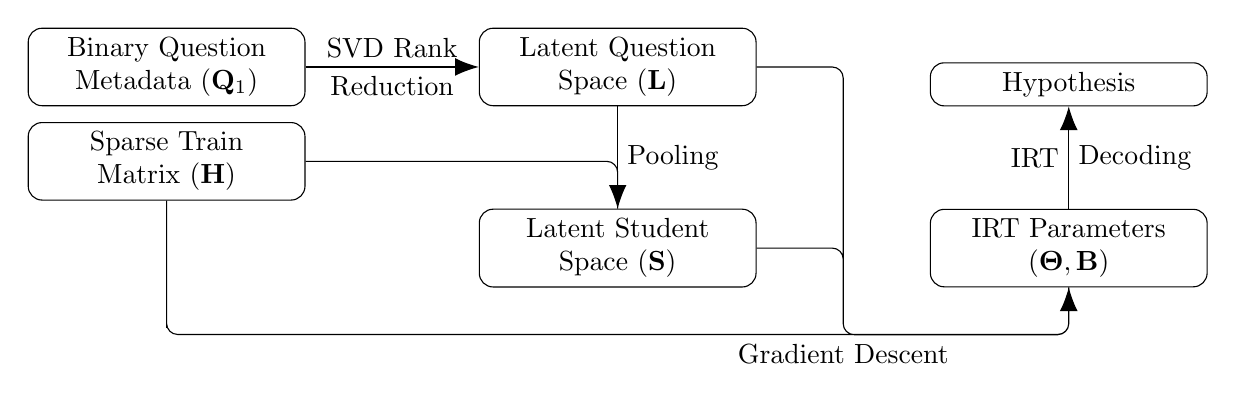
\begin{tikzpicture}[
        auto,
        node distance = 11mm and 22mm,
        base/.style = {draw, rounded corners=5pt,
                       minimum height=1.5em, align=center},
        block/.style = {base, minimum width=10em},
        ]
        \coordinate (in);
        \node [block,right=of in] (A) {Binary Question\\Metadata ($\mathbf{Q}_1$)};
        \node [block,right=of A ] (B) {Latent Question\\Space ($\mathbf{L}$)};
        \node [block,below=2mm of A ] (C) {Sparse Train\\Matrix ($\mathbf{H}$)};
        \node [block,below=13mm of B ] (D) {Latent Student\\Space ($\mathbf{S}$)};
        \node [block,right=of D] (E) {IRT Parameters\\
            ($\mathbf{\Theta},\mathbf{B}$)};
        \node [block,above=13mm of E] (F) {Hypothesis};

        \draw [-{Latex[length=3mm]}, rounded corners] 
            (A) edge ["SVD Rank", "Reduction"']            (B)
            (B) edge ["Pooling"]                  (D)
            (E) edge ["IRT", "Decoding"'] (F)
            (C.east) -|                 (D)
            (B.east) -|  +(11mm,-34mm) -| (E)
            (D.east) -|  +(11mm,-11mm) -| (E)
            (C.south) |- +(0,-17mm) -|
                node[pos=0.375, auto=right]{Gradient Descent}  (E);
    \end{tikzpicture}
    \caption{General architecture of the proposed learning algorithm.}
    \label{fig:architecture}
\end{figure*}

Motivated by our desire to create a latent space, we lay out our architecture
in Figure \ref{fig:architecture}.

We start by constructing the latent space (which we will say has dimension $k$
from now on) with the question metadata. Each question has 388 subjects it can
be a part of, and so has 388 features. We take our question metadata $Q$ and we
encode the features into a binary representation, giving us a binary question
metadata matrix $\mathbf{Q}_1$ of shape $|q| \times |s| = 1774 \times 388$,
where $|q|$ is the number of questions and $|s|$ is the number of subjects. To
construct our latent question matrix $\mathbf{L}$ ($|q| \times k$), we do SVD
rank reduction $\mathbf{Q}_1$. That is:

\begin{align}
    \mathbf{Q}_1 &= \mathbf{U}\mathbf{\Sigma}\mathbf{V}^*\\
    \mathbf{L} &= \mathbf{U}_k\mathbf{\Sigma}_k
\end{align}

Where $\mathbf{U}$ and $\mathbf{V}$ are the left- and right-singular matrices
respectively, and $\mathbf{\Sigma}$ is the eigenvalue matrix. The $k$ subscript
means the matrix has been truncated. This formulation falls out from the shapes
of the matrices, but it also means that $\mathbf{L}$ is exactly the PCA score
matrix, which we are interpreting as a dimensionality reduction from $|s|$ to
$k$. over the rows of $\mathbf{Q}_1$

Next we construct the latent student/user matrix $\mathbf{S}$ of shape $|u|
\times k$ where $|u|$ is the number of users/students. We use the intuition
that the $k$ features of rows of $\mathbf{L}$ represent information about the
skillset required to answer the question corresponding to the given row. If a
student answers every question with a certain feature correct, then we will
want their magnitude in that feature to be very high. If a student gets half
right and half wrong, we will want it to cancel out and for their magnitude in
that feature to be very low. A naïve way of getting these traits is to, for each student, pool over the latent question matrix $\mathbf{L}$ based on how they answered the question. To be precise, we use mean-pooling in the form:

\begin{align}
    \mathbf{S}_i = \frac{\sum_{j}^{} \mathbb{I}[\mathbf{H}_{ij} \ne \text{NaN}]
        (-1)^{\mathbf{H}_{ij} + 1}\mathbf{L}_{ij}}
        {\sum_{j}^{} \mathbb{I}[\mathbf{H}_{ij} \ne \text{NaN}]}
\end{align}

Where $\mathbb{I}$ is the indicator function.

$\mathbb{S}$ and $\mathbb{L}$ now hold the information we want to put into IRT,
but do not relate to each other in a way that would let us put it right into
our IRT evalutation function. Therefore, we first want to learn a mapping to
IRT compatible matrices $\mathbf{\Theta}$ and $\mathbf{B}$ respectively. We set
up the simplest such mapping:

\begin{align}
    \mathbf{\Theta} &= \mathbf{S} \mathbf{W}_\theta \\
    \mathbf{B} &= \mathbf{S} \mathbf{W}_\beta
\end{align}

Were $\mathbf{W}_\theta$ and $\mathbf{W}_\beta$ are matrices we will learn
using gradient descent. One would probably get much better results if using a
neural-network, or some other more sophisticated form of mapping, but we stick
to simplicity here.

For our gradient descent, we minimize negative log-likelihood on the cosine
similarity between $k$ dimensional vectors, similar to the treatment of IRT.

\begin{gather}
    \theta_i = \mathbf{S}_i \mathbf{W}_\theta,
    \beta_j = \mathbf{S}_i \mathbf{W}_\beta \\
    c_{ij} = \frac{\theta_i \beta_j}
        {\lVert\theta_i\rVert_2 \lVert\beta_j\rVert_2} \\
    g_{ij} = \sigma(ac_{ij} + b) \\
    \ell = - \sum_{i,j} \left[\mathbf{H}_{ij} \log g_{ij}
        (1 - \mathbf{H}_{ij}) \log (1 - g_{ij})\right] \\
    \frac{\partial\ell}{\partial\mathbf{W}_\theta} = 
        \frac{\partial\ell}{\partial\mathbf{\Theta}}
        \frac{\partial\mathbf{\Theta}}{\partial\mathbf{W}_\theta} =
        \mathbf{S}^\top
        \frac{\partial\mathbf{\Theta}}{\partial\mathbf{W}_\theta} \\
    \frac{\partial\mathbf{\Theta}}{\partial\mathbf{W}_\theta} =
        \left[\frac{\partial\theta_i}{\partial\mathbf{W}_\theta}\right]_i \\
    \frac{\partial\theta_i}{\partial\mathbf{W}_\theta} =
    \sum_j \left(g_{ij} - H_{ij}\right)
        \left(\frac{\beta_i}{\lVert\theta_i\rVert_2 \lVert\beta_j\rVert_2}
         - c_{ij}\frac{\theta_i}{\lVert{\theta_i}\rVert_2^2}\right)
\end{gather}


Where $\lVert\cdot\rVert_2$ is the $L^2$ norm, and $\sigma$ is the sigmoid
activation function. For the last line, a similar result holds exchanging
$\theta_i$ for $\beta_j$. $a$ and $b$ are parameters the model trains along
with $\mathbf{W}_\theta$ and $\mathbf{W}_\beta$ to prevent the sigmoid from
getting clustered too heavily around 0.5, since the cosine similarity outputs
small values.

We run gradient descent for 10,000 steps, using a learning rate of $1e^{-3}$
for everything except $a$ for which we use a learning rate of $1e^{-4}$. We
initialize the $\mathbf{W}$ matrices using a normal distribution centered
around 0 with a variance of 2 (we tuned this variance as a hyperparameter). We
start $a$ at 5 and $b$ at 0.

\begin{figure}[!ht]
    \centering
    \includesvg[width=\linewidth]{partb_k_search_by_40}
    \captionof{figure}{$k^*$ search for SVD rank reduction based on final
        accuracies of valid}
    \label{fig:kstar}
\end{figure}

For the dimension $k$ of our latent space, we did a hyperparameter search and
found that $k^* = 320$ was optimal. In Figure \ref{fig:kstar} we see the graph
of the search with increments of 40. Not shown is another search which we
repeated at increments of 10 zoomed in around 320 which also showed 320 to be
optimal.

\begin{figure}[!ht]
    \centering
    \includesvg[width=\linewidth]{partb_training_pre_dropout}
    \captionof{figure}{$k^*$ search for SVD rank reduction based on final
        accuracies of valid}
    \label{fig:predropout}
\end{figure}

Figure \ref{fig:predropout} shows the first round of training we did. The blue
line shows us the value of $\ell$ on the train set, and the red line shows us
the "score" (which is the same as for IRT) on the valid set. This got
accuracies of 79.9\% for train, and 64.8\% for both valid and test. This is
less than we hoped for, and as can be seen in the figure, shows clear signs of
overfitting.

\begin{figure}[!ht]
    \centering
    \includesvg[width=\linewidth]{partb_training_with_dropout}
    \captionof{figure}{$k^*$ search for SVD rank reduction based on final
        accuracies of valid}
    \label{fig:withdropout}
\end{figure}

To fix this, we added dropout on $\mathbf{B}$ and $\mathbf{B}$ at a 30\%
chance, which leads to the training curve in \ref{fig:withdropout}. This fixed
the problem, and by doing early stopping based on the valid score we got a
final train accuracy of 72.0\%, valid accuracy of 66.9\%, and test accuracy of
66.6\%.

\end{document}
